\chapter{Contexto Tecnológico}
\label{chap:contexto_tecnologico}

\section{Computación autónoma y bucles de control}

Según \cite{ibmcorporationArchitecturalBlueprintAutonomic2006}, la \textbf{computación autónoma} tiene como objetivo dotar a los sistemas de \textbf{autonomía} en su operación; capacidades para gestionarse a si mismos. Es decir, deberán adaptarse a los distintos escenarios que puedan darse durante su ejecución. Con esto, buscamos alcanzar una reducción en el coste de operación y hacer más gestionable la complejidad de los sistemas.

Estas adaptaciones se realizan en base a directivas de alto nivel proporcionadas por un humano: el humano fija los objetivos que el sistema debe alcanzar; y este deberá adaptarse para lograrlo, si es posible. Siguiendo con el ejemplo de la página web, el operador humano podría definir un máximo de carga por cada instancia. Entonces, cuando se supera el umbral, el sistema podría decidir que se requiere una acción correctiva que consista en desplegar nuevas instancias del servicio cuando haya muchos accesos concurrentes. Cuando la carga de los servicios baje, podemos eliminarlas.

Para implementar estas capacidades de adaptación, recurriremos a la teoría de control y el \textbf{bucle de control} (o \emph{feedback loop}). \cite{brunEngineeringSelfAdaptiveSystems2009} Se trata de un proceso iterativo compuesto por cuatro actividades (figura \ref{fig:bucle-control}):

\begin{figure}[h]
  \centering
  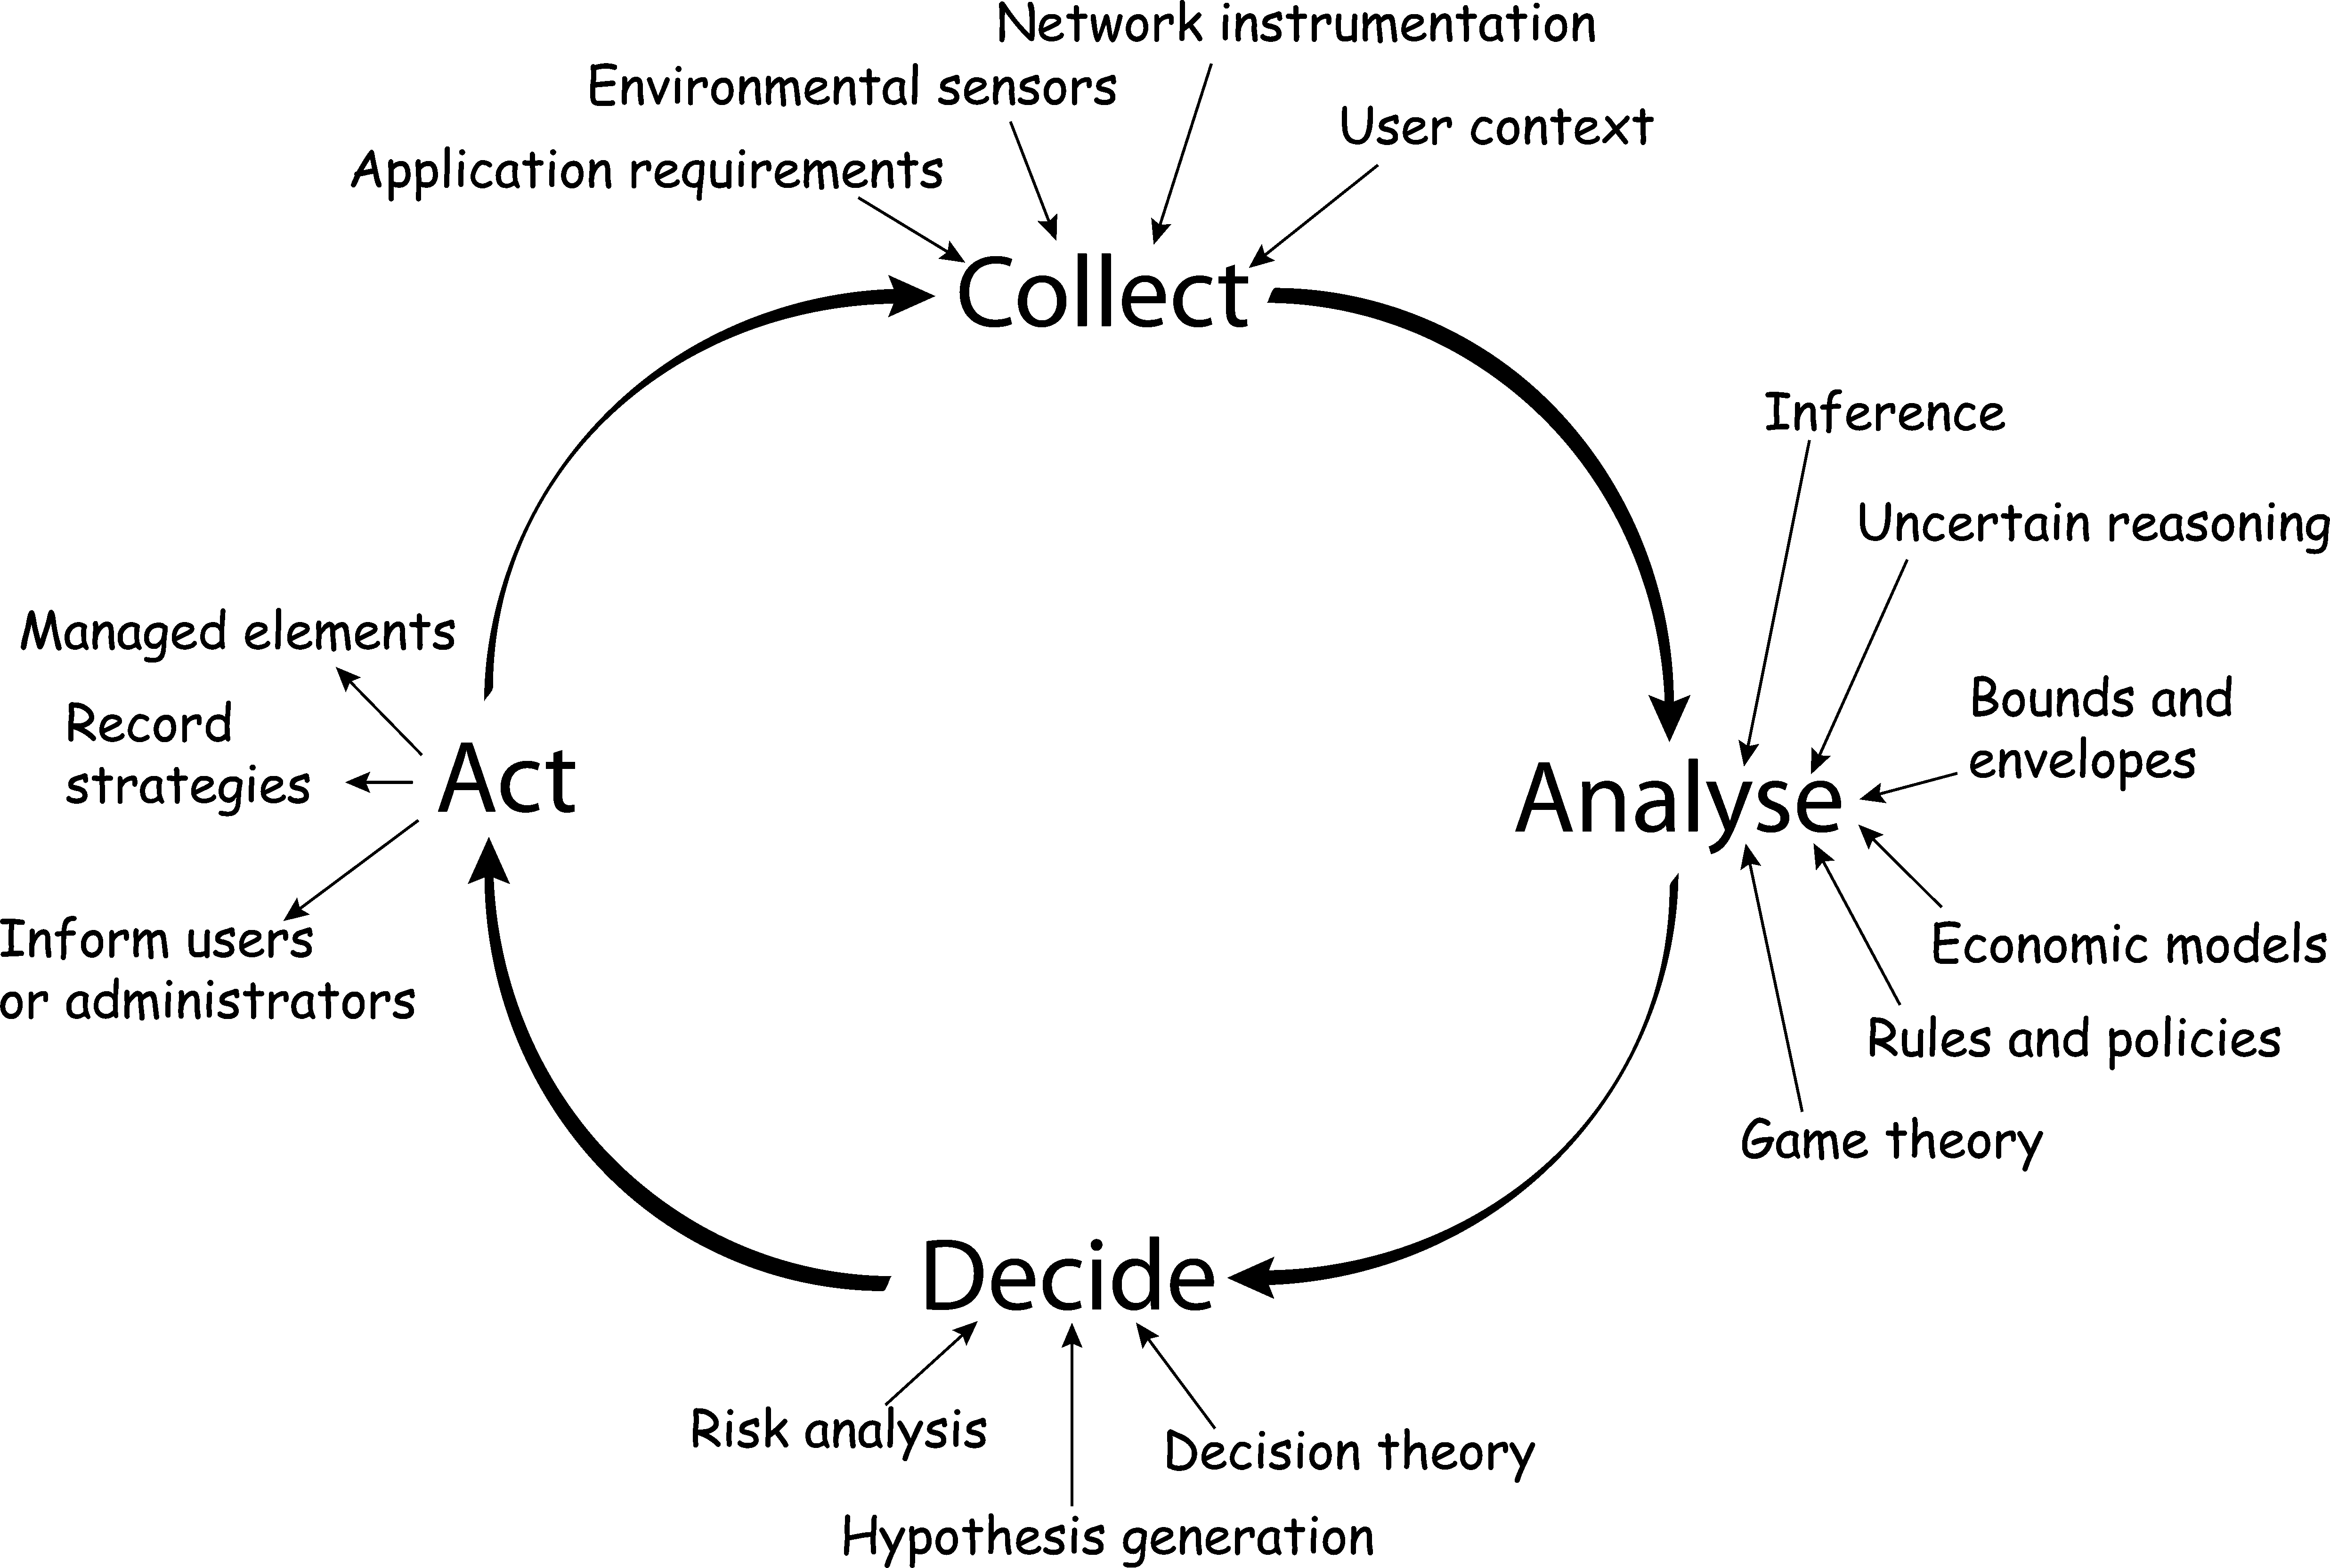
\includegraphics[scale=0.065]{01_introduccion/images/feedback-loop}
  \caption[Un bucle de control genérico. Consta de cuatro actividades: Recopilar información, analizarla, decidir y actuar si procede.]{Un bucle de control genérico. Consta de cuatro actividades: Recopilar información, analizarla, decidir y actuar si procede. Obtenida de \cite{dobsonSurveyAutonomicCommunications2006}.}
  \label{fig:bucle-control}
\end{figure}

\begin{itemize}
  \item \textbf{Recopilar información}: El bucle \textbf{monitoriza} el estado del sistema a través de \textbf{sondas}. Estas reportan información del sistema y del entorno de ejecución. Pueden ser métricas del rendimiento del sistema, estado de los componentes, etc.

  Estos datos en bruto deben ser limpiados, filtrados y agregados. Si se considera que son relevantes, se almacenan para informar las siguientes etapas del bucle.

  \item \textbf{Analizar}: A partir de las propiedades de adaptación, la etapa de análisis debe identificar \textbf{síntomas}: indicadores de una situación que requiera de nuestra atención. Puede ser mediante heurísticas que hayamos configurado, análisis estadístico \textcolor{red}{y cosas así}. Un ejemplo de síntoma sería ''uso de CPU elevado'', ''número elevado de mensajes encolados en un sistema de mensajería'' \textcolor{red}{entre otras}.

  \item \textbf{Decidir}: A partir de los síntomas, el bucle debe determinar si es necesario tomar alguna acción correctiva. \textbf{Planifica} las acciones que se llevarán a cabo para que el sistema se adapte y alcance una configuración deseable. Por ejemplo, si hay muchos mensajes encolados, se podría solicitar el iniciar otra instancia del servicio que los consuma y procese en paralelo.

  \item \textbf{Actuar}: Si el bucle ha planificado alguna acción, se intentará \textbf{ejecutar} en esta etapa final. Mediante \textbf{efectores} en el sistema, el bucle es capaz de cambiar la configuración actual del mismo. Dependiendo del éxito de esta etapa, la adaptación se lleva a cabo o no. Finalizada esta, se vuelve a recopilar información y el bucle continúa iterando.
\end{itemize}

Este tipo de proceso está presente en gran variedad de contextos como puede ser operación de plantas industriales, en procesos naturales, etc. \textcolor{red}{Citar TFM planta embalaje}.

El bucle del control trabaja con un modelo del sistema de alto nivel \cite{garlanIncreasingSystemDependability2003}. Esto le permite definir las adaptaciones desacoplándose de los elementos. Los sistemas adaptativos se basan principalmente en bucles de control. trabajan sobre system models - and in particular, architectural models - are maintained at run time
and used as a basis for system reconfiguration and repair \cite{garlanIncreasingSystemDependability2003}

En la ingeniería de \emph{software}, encontramos diversas aplicaciones de los bucles de control. Pero normalmente están implícitos en la implementación. \cite{brunEngineeringSelfAdaptiveSystems2009}
los bucles de control pueden ser implícitos, dentro del código y las condiciones, o explicitos. \cite{brunEngineeringSelfAdaptiveSystems2009} Lo ideal es contar con bucles externos, esto nos permite separar la funcionalidad de las capacidades de adaptación. \ Esto facilita la implementación.

Garlan et al. also advocate to make self-adaptation external, as opposed to internal or hard-wired, to separate the concerns of system
functionality from the concerns of self-adaptation [9,16].

\textcolor{red}{Hablar de agentes autónomos como aplicación práctica. \cite{savaglioAgentbasedInternetThings2020}}

\subsection{Arquitectura para sistemas autónomos: Bucles MAPE-K}

Un estilo arquitectónico muy representativo de este tipo de sistemas es el basado en bucles MAPE-K \cite{ibmcorporationArchitecturalBlueprintAutonomic2006, fonsServiciosAdaptivereadyPara2021} de IBM. Se trata de una arquitectura para sistemas distribuidos autónomos, que requieran del mínimo de intervención humana para operar. Nace con el objetivo de definir e implementar sistemas autoadaptativos.

Estos sistemas ser capaces de auto-gestionarse en base a \textbf{políticas}. Las políticas son un conjunto de objetivos de alto nivel que definen los usuarios encargados del sistema. El sistema debe tratar de alcanzarlos durante su funcionamiento. Además, estos motivan los cambios en el sistema, que trata de adaptarse para alcanzarlos.

Su componentes principales son los \textbf{elementos autónomos}. Cada uno de estos es capaz de autogestionarse, y colaborar en conjunto con el resto de elementos autónomos de la arquitectura para alcanzar los objetivos. \textcolor{red}{¿Agent based?} Además, son elementos ''componibles'': podemos ''apilarlos'' uno encima del otro. De ahí surge el concepto de bucle orquestador.

Los elementos autónomos, a su vez, pueden dividirse en dos partes: los recursos manejados y un manejador autónomo (el bucle de control).

Los \textbf{recursos manejados} son las unidades de funcionalidad del sistema. Puede ser cualquier tipo de recurso, \emph{hardware} o \emph{software}. Para dotarlas de capacidad de autoadaptación, las emparejamos con un \textbf{manejador autónomo}. El bucle de control. Se trata de un bucle de control externo, utilizado para dotar de capacidades autónomas a sistemas. Gestiona al recurso en base a la información que recoge del entorno de ejecución y las políticas que guían su adaptación.

Para poder monitorizar el recurso, y poder evaluar métricas cómo su estado o su desempeño, debemos \textbf{instrumentar} el recurso manejado. Debemos implementar \textbf{sondas} en nuestro servicio que reporten datos relevantes a los monitores del bucle.

En la figura \ref{fig:autonomic-element} tenemos una representación de un elemento autónomo. Distinguimos las dos partes: el manejador y el recurso. El manejador está acoplado al recurso a través de sus sensores y efectores. Además, podemos observar que el propio manejador expone sensores y efectores, lo que permiten ser controlador por manejadores autónomos orquestadores.

Estos gestionan a un nivel superior uno o más elementos autonómicos.

\begin{figure}[h]
  \centering
  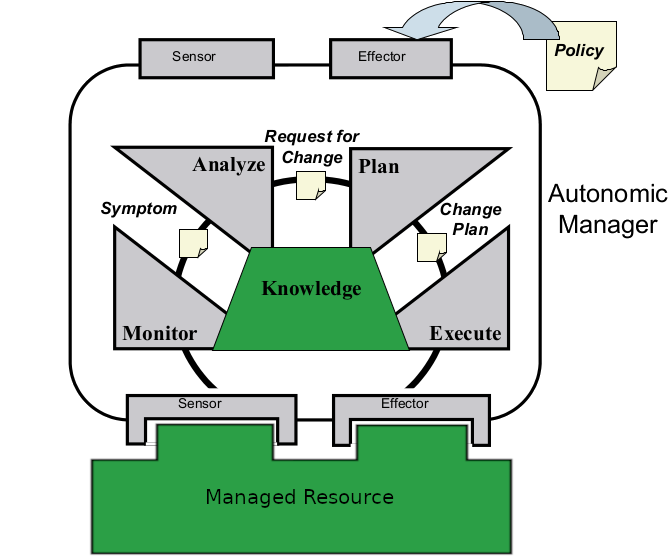
\includegraphics[scale=2]{02_contexto_tecnologico/images/autonomic-element}
  \caption[Representación de un elemento autónomo. Distinguimos el recurso manejado y el manejador autónomo. Bucle MAPE-K (Monitor, Analysis, Planification, Execution and Knowledge)]{Representación de un elemento autónomo. Distinguimos el recurso manejado y el manejador autónomo. Bucle MAPE-K (Monitor, Analysis, Planification, Execution and Knowledge). Basada en imagen de \cite{ibmcorporationArchitecturalBlueprintAutonomic2006}.}
  \label{fig:autonomic-element}
\end{figure}

El recurso manejado puede ser un sistema \emph{hardware} o \emph{software} cualquiera. El único requisito es que debe implementar los \textbf{\emph{touchpoints}} (\textcolor{red}{puntos de contacto?}): interfaces que permiten al bucle de control obtener información del estado del sistema y cambiar su configuración en base a las políticas. Hay dos tipos de \emph{touchpoints}: \textbf{sondas} y \textbf{efectores}.

Las sondas reportan al bucle información del estado del sistema. Puede ser cualquier tipo de métrica que queramos controlar. Por ejemplo, \emph{health checks}, información de salud de la aplicación; propiedades del sistema que queramos controlar.

Por otro lado, los efectores, nos ayudan a modificar el estado del sistema manejado. Pueden ser ficheros de configuración, comandos, etc.

En la figura \ref{fig:autonomic-element} podemos apreciar que el bucle puede dividirse en 5 componentes distintos: \cite{ibmcorporationArchitecturalBlueprintAutonomic2006}

\begin{itemize}
  \item \textbf{Base de conocimiento}: almacena el conocimiento relevante para la operación del bucle de control. Es tanto información del sistema como información del entorno de operación. Cada una de las claves almacenadas se conoce también como \textbf{propiedad de adaptación}.

  El conocimiento se comparte entre todos los componentes del bucle de control.

  \item \textbf{Monitor}: Recibe mediciones de las sondas del recurso manejado. Se encarga de recoger, agregar y filtrar estas mediciones para determinar si ha ocurrido un evento relevante que deba ser reportado. Por ejemplo, si la temperatura de una habitación supera un umbral definido por el usuario.

  Estos datos en bruto deben ser limpiados, filtrados y agregados. Si se considera que son relevantes, se traducen a \textbf{propiedades de adaptación}: conjunto de propiedades que describen el modelo del estado pasado y actual de nuestro sistema \cite{garlanIncreasingSystemDependability2003}. Su principal función es informar las siguientes etapas del bucle.

  \item \textbf{Analizador}: Conjunto de \textbf{reglas de adaptación} que se suscriben a las propiedades de adaptación. Están compuestas una condición y una acción. Cada vez que cambie alguna de las propiedades de las que dependen, se evalua su condición. Si esta se cumple, se ejecuta la acción asociada, que suele ser una propuesta de cambio en la configuración del sistema.

  \item \textbf{Planificador}: Si se ha llegado a ejecutar alguna regla de apdatación, el planificador recoge sus propuestas de cambio y determina las acciones necesarias para cumplir el objetivo. Basándose en las \textbf{políticas} de operación y los \textbf{objetivos} del sistema,

  \item \textbf{Ejecutor}: Recibe se traducen las acciones de alto nivel solicitadas en el modelo a acciones de bajo nivel.
\end{itemize}
